The companion Python module to this paper \texttt{sort\_analysis.py} was written to verify experimentally the aforementioned theoretical results.

\begin{figure}
    \centering
    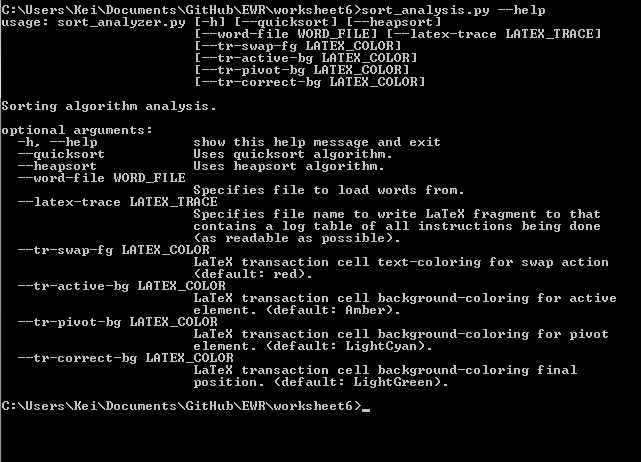
\includegraphics[width=0.95\linewidth]{images/help_command.png}
    \caption{Screenshot of the help command.}
\end{figure}

The user can select the desired algorithm by using \texttt{--quicksort} or \texttt{--heapsort} and specifiying the path to a text file containing words separated by spaces (see figure \ref{fig:quicksortdemo} and \ref{fig:heapsortdemo}).

\begin{figure}
    \centering
    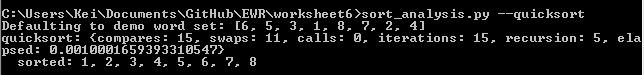
\includegraphics[width=0.95\linewidth]{images/quicksort_demo.png}
    \caption{Screenshot of quicksort demonstration.}\label{fig:quicksortdemo}
\end{figure}
\begin{figure}
    \centering
    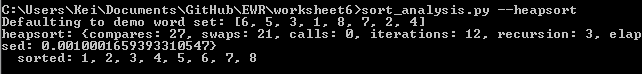
\includegraphics[width=0.95\linewidth]{images/heapsort_demo.png}
    \caption{Screenshot of heapsort demonstration.}\label{fig:heapsortdemo}
\end{figure}

\texttt{--latex\_trace} outputs a latex file documenting the steps of the algorithms as readable as possible.